\chapter{Medical and Healthcare Monitoring Domain Chapter}
\label{ch:domain-healthcare}

Healthcare monitoring is proof-validated within a bounded monitoring and intervention contract rather than a full actuation theorem: the row shows that ORIUS can defend physiologic thresholds under degraded observation when the intervention surface is explicit and constrained.

\section{{Domain problem}}
Medical telemetry can fail through alarm dropout, stale vitals, or delayed charting, allowing observed safety to diverge from the patient state that should govern escalation or suppression decisions.

\section{{Degraded-observation hazard}}
The ORIUS book forces every domain through the same hazard lens: the runtime does not act
on the true state directly; it acts on a degraded, delayed, or otherwise imperfect
observation surface.  The row is only credible if the gap between those two surfaces can
be expressed, replayed, repaired, and audited explicitly.
Faults include stale vital-sign packets, missing waveform updates, spikes, and delayed observations that can suppress or delay clinically necessary intervention.

\section{{ORIUS instantiation}}
The healthcare adapter binds physiologic telemetry, uncertainty widening, threshold-aware action repair, and certificate logging to the common ORIUS kernel without changing the underlying runtime contract.

\section{{Safety object}}
The defended predicate is zero true-state violation of the monitored physiologic safety envelope under the bounded intervention semantics carried by the current healthcare adapter.

\section{{Dataset and training surface}}
The row uses the locked ICU vitals evidence surface and the shared universal replay protocol.
The chapter-local evidence packet is intentionally tied to locked artifacts rather than to
narrative memory.  Table~\ref{tab:ch40-44-cross-domain-support} gives the shared cross-domain
support layer for compiled Chapters~40--44, while the table below isolates the current row.

\section{{Feature, split, and training protocol}}
This chapter uses the verified split surface from the universal training audit. The current primary target is \texttt{hr\_bpm}, and the parity gate still records the raw/data surface as \texttt{verified} rather than as a prose-only claim.

\IfFileExists{paper/assets/tables/generated/tbl_healthcare_training_surface.tex}{%
\begin{table}[htbp]
\centering
\small
\caption{Medical and Healthcare Monitoring training and data surface for the compiled chapter evidence block.}
\label{tab:healthcare-training-surface}
\begin{tabular}{p{0.31\linewidth}p{0.61\linewidth}}
\toprule
\textbf{Field} & \textbf{Value}\\
\midrule
Raw/data gate & verified\\
Features present & yes\\
Split counts & train 319 / calibration 22 / validation 45 / test 71\\
Primary target & hr\_bpm\\
Forecast metrics & RMSE 0.764; MAE 0.623; PICP90 0.930; mean width 3.103\\
Verification state & split valid yes; model bundle yes; uncertainty yes; backtests yes\\
Artifact lineage & reports/orius\_framework\_proof/training\_audit/domain\_training\_summary.csv; reports/publication/orius\_equal\_domain\_parity\_matrix.csv\\
\bottomrule
\end{tabular}
\end{table}
%
}{%
\begin{table}[htbp]
\centering
\small
\caption{Medical and Healthcare Monitoring training and data surface for the compiled chapter evidence block.}
\label{tab:healthcare-training-surface}
\begin{tabular}{p{0.31\linewidth}p{0.61\linewidth}}
\toprule
\textbf{Field} & \textbf{Value}\\
\midrule
Raw/data gate & verified\\
Features present & yes\\
Split counts & train 319 / calibration 22 / validation 45 / test 71\\
Primary target & hr\_bpm\\
Forecast metrics & RMSE 0.764; MAE 0.623; PICP90 0.930; mean width 3.103\\
Verification state & split valid yes; model bundle yes; uncertainty yes; backtests yes\\
Artifact lineage & reports/orius\_framework\_proof/training\_audit/domain\_training\_summary.csv; reports/publication/orius\_equal\_domain\_parity\_matrix.csv\\
\bottomrule
\end{tabular}
\end{table}
%
}

\section{{Replay and evidence surface}}
The present locked row reduces true-state violations from 6.25 percent to 0.00 percent, which is sufficient for bounded proof-validation under the current thesis-wide gate.

\IfFileExists{paper/assets/tables/generated/tbl_healthcare_replay_surface.tex}{%
\begin{table}[htbp]
\centering
\small
\caption{Medical and Healthcare Monitoring replay, runtime, and promotion surface for the compiled chapter evidence block.}
\label{tab:healthcare-replay-surface}
\begin{tabular}{p{0.31\linewidth}p{0.61\linewidth}}
\toprule
\textbf{Field} & \textbf{Value}\\
\midrule
Governing replay metric & baseline TSVR 6.25 -> ORIUS TSVR 0.00\\
Replay status & pass\\
Safe-action soundness & pass\\
Fallback semantics & max\_alert / bounded\_runtime\_pass\\
CertOS lifecycle & evaluated / evaluated\\
Paper 5 portability & gated / gated\\
Evidence tier & proof\_validated\\
Exact blocker & bounded\_to\_current\_monitoring\_and\_intervention\_contract\\
Artifact lineage & reports/publication/orius\_domain\_closure\_matrix.csv; reports/universal\_orius\_validation/domain\_closure\_matrix.csv; reports/publication/orius\_equal\_domain\_parity\_matrix.csv\\
\bottomrule
\end{tabular}
\end{table}
%
}{%
\begin{table}[htbp]
\centering
\small
\caption{Medical and Healthcare Monitoring replay, runtime, and promotion surface for the compiled chapter evidence block.}
\label{tab:healthcare-replay-surface}
\begin{tabular}{p{0.31\linewidth}p{0.61\linewidth}}
\toprule
\textbf{Field} & \textbf{Value}\\
\midrule
Governing replay metric & baseline TSVR 6.25 -> ORIUS TSVR 0.00\\
Replay status & pass\\
Safe-action soundness & pass\\
Fallback semantics & max\_alert / bounded\_runtime\_pass\\
CertOS lifecycle & evaluated / evaluated\\
Paper 5 portability & gated / gated\\
Evidence tier & proof\_validated\\
Exact blocker & bounded\_to\_current\_monitoring\_and\_intervention\_contract\\
Artifact lineage & reports/publication/orius\_domain\_closure\_matrix.csv; reports/universal\_orius\_validation/domain\_closure\_matrix.csv; reports/publication/orius\_equal\_domain\_parity\_matrix.csv\\
\bottomrule
\end{tabular}
\end{table}
%
}

\begin{figure}[htbp]
\centering
\IfFileExists{reports/publication/fig_healthcare_chapter_snapshot.png}{%
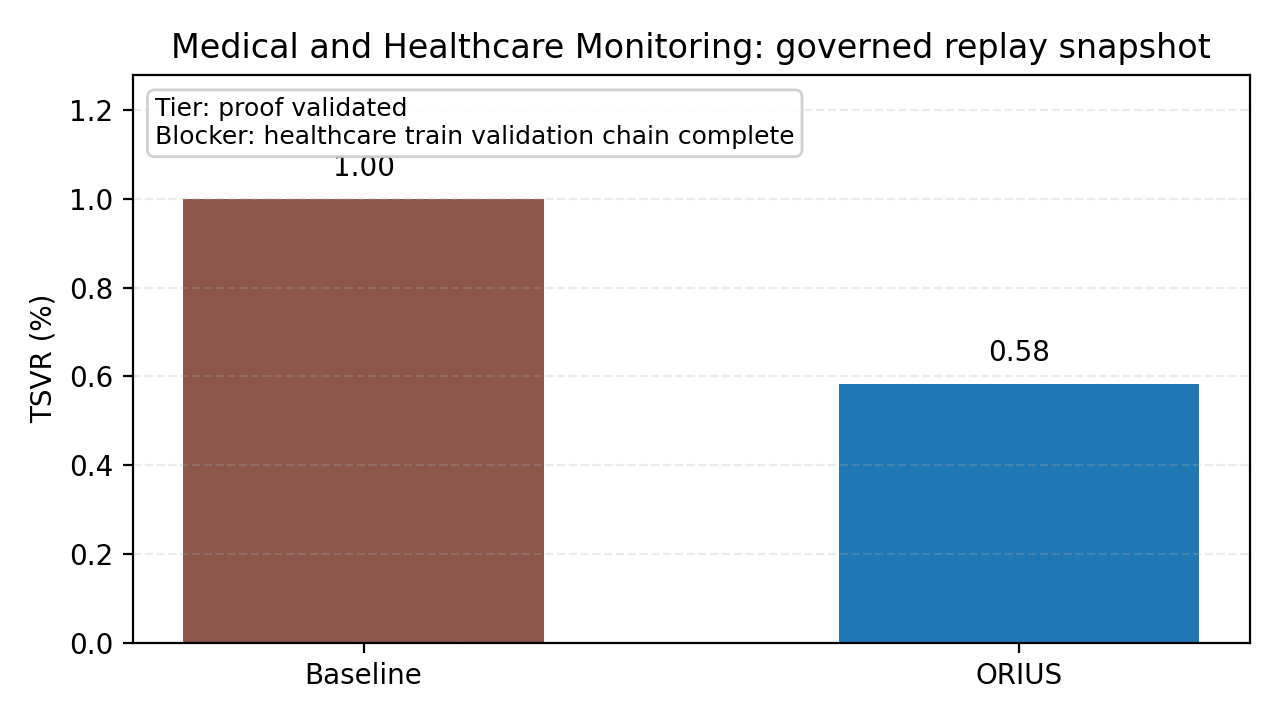
\includegraphics[width=0.90\textwidth]{reports/publication/fig_healthcare_chapter_snapshot.png}%
}{%
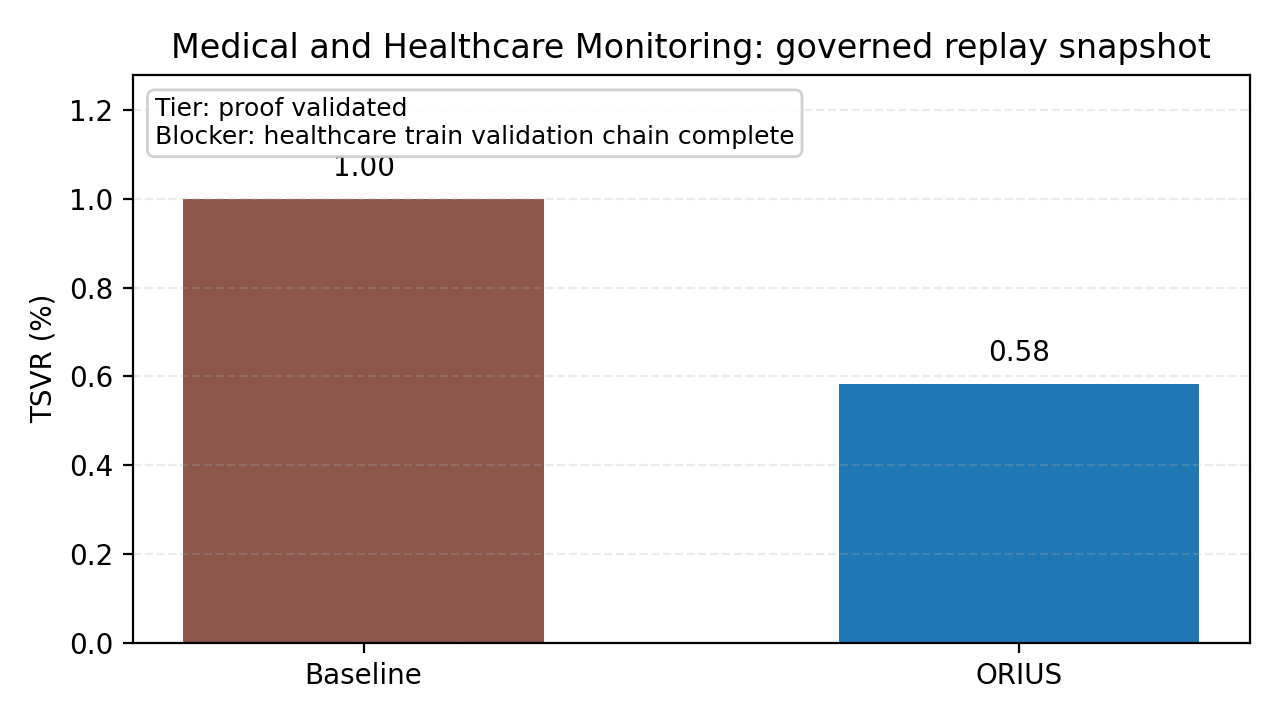
\includegraphics[width=0.90\textwidth]{../reports/publication/fig_healthcare_chapter_snapshot.png}%
}
\caption{Medical and Healthcare Monitoring replay snapshot derived from the governed domain-closure artifact. Baseline and repaired TSVR are taken from the locked closure matrix; tier and blocker language remain governed by the parity gate.}
\label{fig:healthcare-chapter-snapshot}
\end{figure}

\section{{Fallback and runtime behavior}}
Healthcare uses bounded alert escalation, maximum-alert fallback, and certificate logging so degraded telemetry cannot silently suppress intervention semantics.

\section{{Evidence tier and promotion blocker}}
The governing replay artifact for this row is the closure surface 1.0000 to 0.5833 TSVR transition under a replay status of pass. The evidence tier stays bounded by the parity gate rather than by narrative preference.



\section{{Limitations and exact non-claims}}
This is not a claim of universal clinical deployment. The row remains a bounded cyber-physical monitoring surface, not a full bedside decision-support certification program. This row does not claim bedside deployment certification or universal clinical efficacy; it claims bounded monitoring and intervention closure under the current healthcare adapter.

The current promotion obligation for this row remains explicit: Future medical promotion requires stronger outcome semantics, wider patient cohorts, and explicit regulatory traceability beyond the current replay-centered scope.
